\documentclass[tikz,border=10pt]{standalone}


\begin{document}
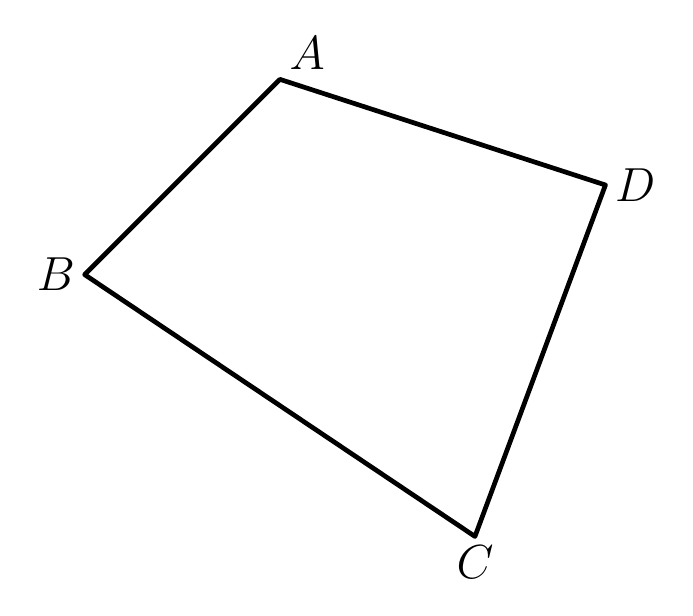
\begin{tikzpicture}
\coordinate (A) at (-0.845,2.923);
\coordinate (B) at (-3.325,0.443);
\coordinate (C) at (1.632,-2.882);
\coordinate (D) at (3.289,1.581);

  
  \draw[line width=1.7pt, line join=round] (A) -- (B) -- (C) -- (D) -- cycle;
  
  \node[above right, font=\fontsize{17}{20.4}\selectfont] at (A) {$A$};
  \node[left, font=\fontsize{17}{20.4}\selectfont] at (B) {$B$};
  \node[below, font=\fontsize{17}{20.4}\selectfont] at (C) {$C$};
  \node[right, font=\fontsize{17}{20.4}\selectfont] at (D) {$D$};
\end{tikzpicture}
\end{document}